\documentclass[12pt]{beamer}
\usetheme{CambridgeUS}
\usepackage[utf8]{inputenc}
\usepackage[german]{babel}
\usepackage[T1]{fontenc}
\usepackage{amsmath}
\usepackage{amsfonts}
\usepackage{amssymb}
\usepackage{graphicx}

\author{Philipp Hörauf und Toni Bartsch}
\title{DIY: Carbonwickelmaschine}

\beamertemplatenavigationsymbolsempty
%\setbeamercovered{transparent} 
%\setbeamertemplate{navigation symbols}{} 
%\logo{}  %Dickbutt!
%\institute{} 
\date{\today} 
\subject{DIY-Vorlesung} 

\begin{document}


\begin{frame}
\titlepage
\end{frame}


\begin{frame}
\tableofcontents
\end{frame}

\section{Motivation}
\begin{frame}{Motivation}
\subsection{Vielfältige Verwendbarkeit von Carbonrohren}
Bisher gibt es keine OpenSource Wickelmaschine\newline
\vspace{1cm}
Carbonrohre sind...
\begin{itemize}
	\item extrem leicht
	\item verwindungssteif
	\item korrosionsbeständig
	\item quasi immun gegen Wärmeausdehnung
\end{itemize}
\vspace*{1cm}

Daher ist Carbon ideal für leichte und zugleich robuste Aufbauten geeignet, z.B. im Modellbau
\end{frame}


\begin{frame}
\subsection{Momentane Situation}
Problem: Carbonrohre können teuer werden, vor allem wenn man größere Mengen oder exotische Maße benötigt.\newline

\begin{figure}
	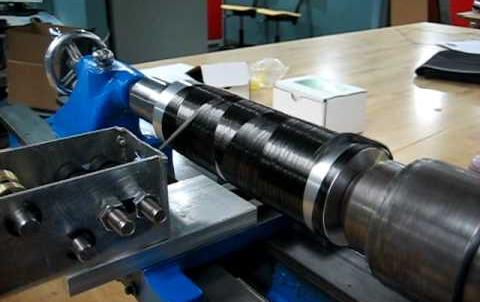
\includegraphics[width=6cm]{./hqdefault.jpg}
	\caption{professionelle Carbonwickelmaschine, \url{http://carbon-deutschland.de}}
\end{figure}

Diese Maschinen sind recht teuer und schwer erhältlich.
\end{frame}


\section{Projektbeschreibung}
\begin{frame}{Projektbeschreibung}
\subsection{Planung und gewünschte Eckdaten}
Daher: Eigenbau einer Carbonwickelmaschine aus Normteilen und selbst Designtem.\newline
\vspace{0.5cm}


voraussichtliche Eckdaten der Maschine:
\begin{itemize}
	\item Maximale Wickellänge 1200\,mm
	\item Größter Durchmesser 250\,mm
	\item Verarbeitung von Carbon- und Glasfasern
	\item Wickelvorgang PC-kontrolliert
	\item Möglichst kostengünstiger Aufbau
\end{itemize}
\end{frame}


\begin{frame}
\subsection{aktuelles 3D-Modell des Prototypen}
Konstruktion und Fertigung der Maschine aus Aluminium und Holz\newline

\begin{figure}
	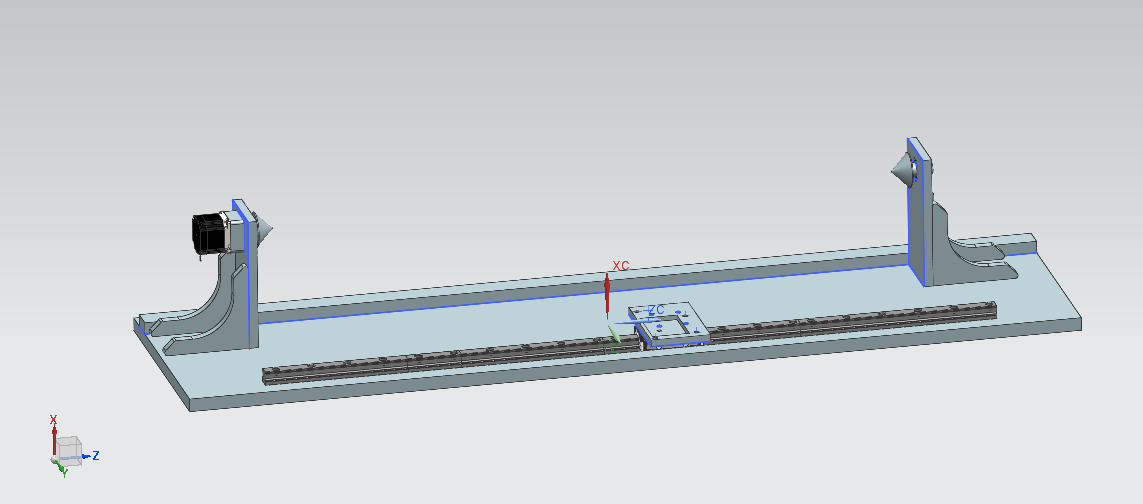
\includegraphics[width=10cm]{./carbonwickler_geschnitten.png}
	\caption{aktueller Screenshot aus Siemens NX}
\end{figure}
\end{frame}


\end{document}